%# -*- coding: utf-8 -*-
\documentclass{ctexart}
%
%页眉页脚

\usepackage{geometry}
\geometry{left=2.5cm,right=2.5cm,top=2.5cm,bottom=2.5cm}
\usepackage{xcolor}
\usepackage{graphicx}
\usepackage{amsmath}
\usepackage{url}
\usepackage{enumerate}
\usepackage{subfigure}
\usepackage{listings} 
\usepackage[colorlinks,linkcolor=black]{hyperref}% 书签
\usepackage{fancyhdr}

\fancyhead[R]{\thepage}% 这是奇数页右页眉、偶数页左页眉
\fancyhead[L]{}
\chead{MATLAB 综合实验之图像处理}%这是中间页眉
\pagestyle{fancy}
\lstset{numbers=left, %设置行号位置
    numberstyle=\tiny, %设置行号大小
    keywordstyle=\color{blue}, %设置关键字颜色
    commentstyle=\color[cmyk]{1,0,1,0}, %设置注释颜色
    frame=single, %设置边框格式
    breaklines, %自动折行
    extendedchars=false, %解决代码跨页时,章节标题,页眉等汉字不显示的问题
    xleftmargin=1.5em,xrightmargin=1.5em, aboveskip=1em, %设置边距
    tabsize=4, %设置tab空格数
    showspaces=false %不显示空格
}
%中文
\usepackage{xeCJK}
%字体设置
\usepackage{indentfirst}
\setlength{\parindent}{2em} %首行缩进
\renewcommand\thesubsection{(\arabic{subsection})}
\renewcommand\thesubsubsection{(\alph{subsubsection})}

\title{MATLAB 综合实验之图像处理\footnote{所有的.m文件均采用utf8编码,windows版matlab中打开可能会出现中文乱码的情况,请用其它编辑器打开}}
\author{聂浩~~ 无31~~ 2013011280}
\date{\today}
\begin{document}
\maketitle
\section{基础知识}
\subsection{
MATLAB 提供了图像处理工具箱,在命令窗口输入 help images 可查看该工具箱内的所有函数。 请阅读并大致了解这些函数的基本功能。}

感觉较为常用的函数有:
\begin{itemize}
    \item{image 建立图片对象,在坐标轴中绘制,颜色取决于现在的颜色设置}
    \item{imshow 显示图片(按照原来图片的大小)}
    \item{imread 读取图片文件}
    \item{imwrite 写图片文件}
    \item{imabsdiff 比较两张图片的差异}
    \item{checkerboard 生成棋盘}
\end{itemize}

\subsection{
利用 MATLAB 提供的 Image file I/O 函数分别完成以下处理:}
\subsubsection{以测试图像的中心为圆心,图像的长和宽中较小值的一半为半径画一个红颜色的圆:}
因为这个图像非常小,所以直接用循环就进行了处理,没有进行太多优化.图像如\ref{1circle},代码见下一问。
\begin{figure}
    \centering
    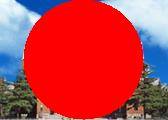
\includegraphics[width=0.3\textwidth]{circle.jpg}\\
    \caption{绘制红色圆\label{1circle}}
\end{figure}

\subsubsection{将测试图像涂成国际象棋状的“黑白格”的样子,其中“黑”即黑色,“白”则意味着保留原图。 用一种看图软件浏览上述两个图,看是否达到了目标。}
因为该图像大小为,$120\times 168$,长宽并不能被8整除,所以两边出现了黑边。图像如\ref{1board}
\begin{figure}
    \centering
    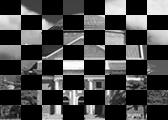
\includegraphics[width=0.3\textwidth]{board.jpg}\\
    \caption{绘制黑白格\label{1board}}
\end{figure}

代码如下(a3\_1.m):
\lstinputlisting[language=matlab]{a3_1.m}

\section{图像压缩编码}
\subsection{
像的预处理是将每个像素灰度值减去128,
这个步骤是否可以在变换域进行?
请在测试图像中截取一块验证你的结论。}
根据二维DCT变换的定义式$C=DPD^T$,这是一个线性变换,所以变换前后处理是一致的。

在这里截取了hall\_gray(61:68,81:88),两种处理次序后的绝对值差在$10^{-12}$数量级,可以认为这只是计算误差,故两者等价。

代码如下(a3\_2\_1.m):
\lstinputlisting[language=matlab]{a3_2_1.m}

\subsection{
请编程实现二维 DCT ,并和 MATLAB 自带的库函数 dct2 比较是否一致。}
我直接使用计算D矩阵然后相乘的方法进行计算,其计算复杂度为$O(n^2)$。

系统的DCT2函数的调用了两次DCT函数,而DCT函数则使用了FFT,因此其计算复杂度为$O(n\log (n)$。

两者的误差在$10^{-12}$数量级,可以认为这只是计算误差。

在数据较大时,如图\ref{a322},系统DCT2函数快于我的my\_DCT2函数。\footnote{因为计算机差异,具体值可能不同}
\begin{figure}
    \centering
    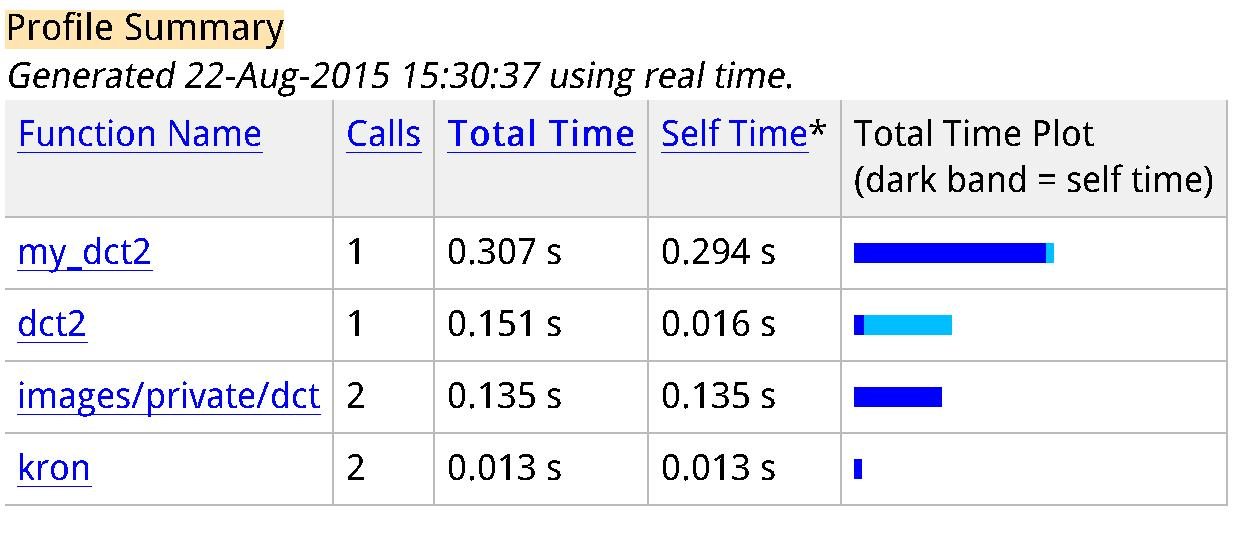
\includegraphics[width=0.8\textwidth]{a3_2_2.jpg}\\
    \caption{将hall\_gray重复100次后两种
    DCT变换所消耗的时间\label{a322}}
\end{figure}

my\_dct2的代码如下:
\lstinputlisting[language=matlab]{my_dct2.m}

测试代码如下(a3\_2\_2.m):
\lstinputlisting[language=matlab]{a3_2_2.m}

\subsection{
如果将 DCT 系数矩阵中右侧四列的系数全部置零,逆变换后的图像会发生什么变化?选取一块图验证你的结论。 如果左侧的四列置零呢?
}
如图\ref{a323},右侧四列都置零,逆变换后的图像变化不大,因为人眼对高频分量不敏感。当左侧四列都置零,逆变换图片变暗。因为很多低频分量,包括基频被滤掉,导致各点值偏小而发暗。
\begin{figure}
    \centering
    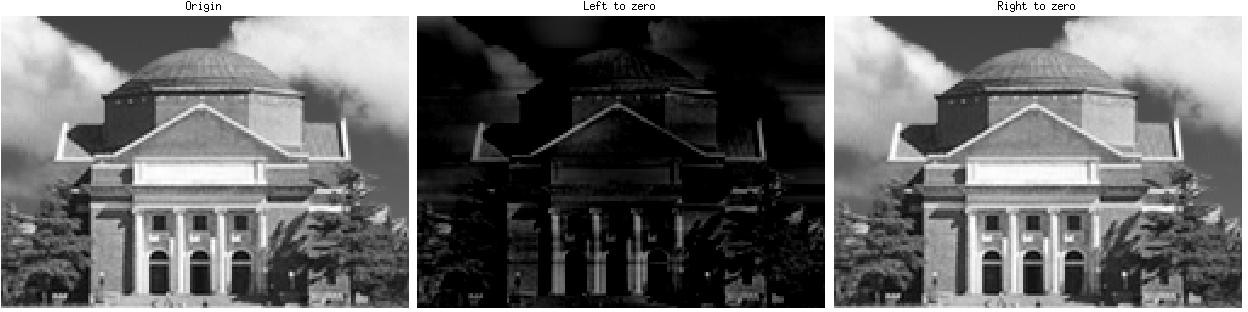
\includegraphics[width=0.8\textwidth]{a3_2_3.jpg}\\
    \caption{左四列与右四列分别清零\label{a323}}
\end{figure}

代码如下(a3\_2\_3.m)
\lstinputlisting[language=matlab]{a3_2_3.m}
\subsection{
若对 DCT 系数分别做转置、 旋转 90 度和旋转 180 度操作 (rot90) ,逆变换后恢复的图像有何变化?选取一块图验证你的结论。}
如图\ref{a324},转置使得图像沿左上至右下的对角线翻转镜像;旋转$90^{\circ}$使图像在之前的基础上还出现了黑白条纹;旋转$180^{\circ}$后图像没有旋转,但是出现了黑白小斑点。

这是因为转置并未改变高低频信息,但两轴被交换,故出现翻转;旋转使得高频和低频分量的信息混淆,故高频相对之前被放大了——旋转$90^{\circ}$只有一个方向的高频较明显,故为条纹;旋转$180^{\circ}$则增强了两个方向的高频分量,故为斑点。
\begin{figure}
    \centering
    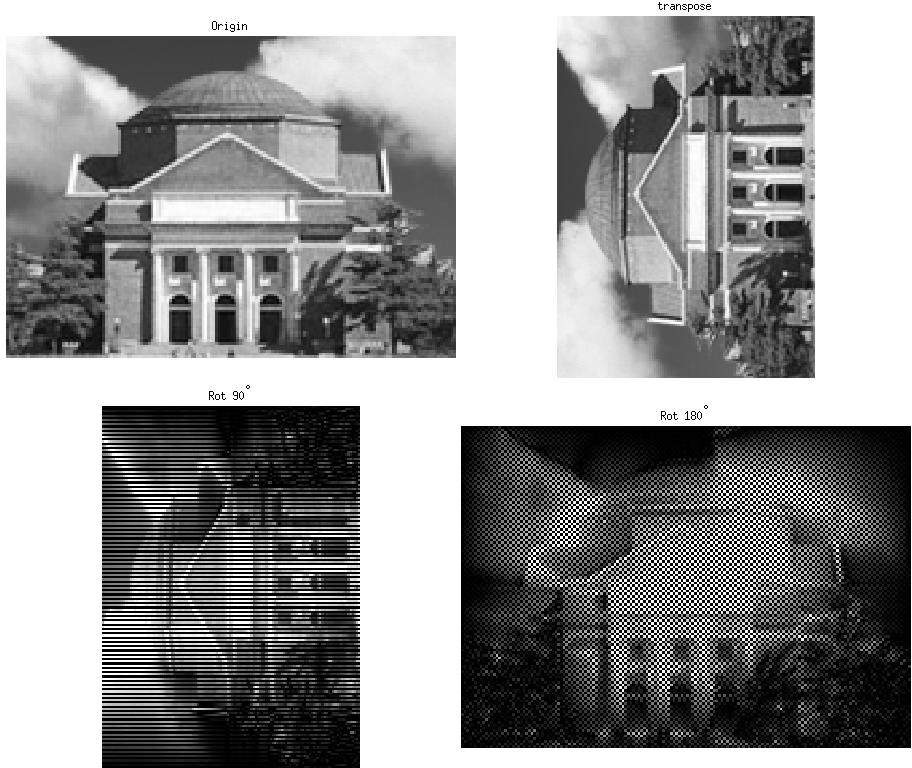
\includegraphics[width=0.8\textwidth]{a3_2_4.jpg}\\
    \caption{左四列与右四列分别清零\label{a324}}
\end{figure}

代码如下(a3\_2\_4.m):
\lstinputlisting[language=matlab]{a3_2_4.m}
\subsection{
如果认为差分编码是一个系统,请绘出这个系统的频率响应,说明它是一个\_\_\_\_(低通、 高通、 带通、带阻)滤波器。 DC 系数先进行差分编码再进行熵编码,说明 DC 系数的\_\_\_\_频率分量更多。}
差分编码的差分方程为$y(n)=x(n-1)-x(n)$,其系统函数为\[H(z)=\frac{1}{z}-1\]仿真得到图\ref{a325},这是一个高通滤波器。说明DC系数的低频分量更多,这样处理可以压缩低频分量。
\begin{figure}
    \centering
    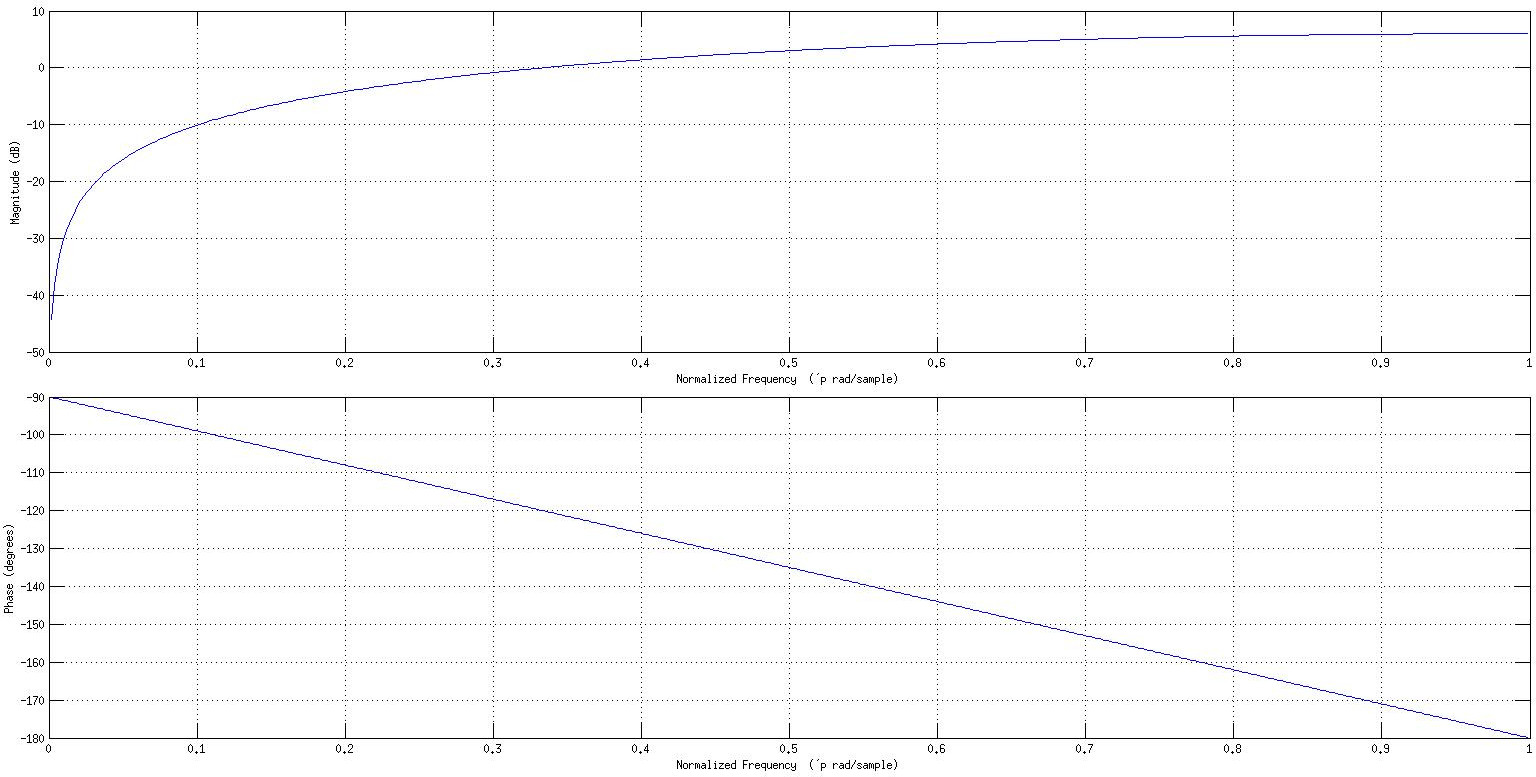
\includegraphics[width=0.8\textwidth]{a3_2_5.jpg}\\
    \caption{差分的频率响应\label{a325}}
\end{figure}
代码如下:{a3\_2\_5.m}
\lstinputlisting[language=matlab]{a3_2_5.m}
\subsection{
DC 预测误差的取值和 Category 值有何关系?如何利用预测误差计算出其 Category?
}

DC的预测误差$\hat{c}_D=0$时,Category=0,否则$Category=ceil(log2(abs(\hat{c}_D)+1))$

\subsection{
 你知道哪些实现 Zig-Zag 扫描的方法?请利用 MATLAB 的强大功能设
计一种最佳方法。
}
按照最原始的思路,采用循环的方式,将元素依次放入一数组中,然后利用逻辑判断决定接下来去哪个元素。但是这样速度显然很低。更为直接的思路是利用查表法,因为该图像大小为$8\times8$,直接构造一个查表矩阵是最好的,同时,通过查询\footnote{参照\url{http://blog.sina.com.cn/s/blog_54e2ed7b0100mmb7.html}},将矩阵转换到一维处理是更为简便的方式,不过其zigzag的顺序和试验要求有一定出入,简单修改即可。

代码如下(zigzag.m):
\lstinputlisting[language=matlab]{zigzag.m}
测试该函数的代码(a\_3\_7.m)
\lstinputlisting[language=matlab]{zigzag.m}

\subsection{
对测试图像分块 DCT 和量化,将量化后的系数写成矩阵的形式,其中每一列为一个块的 DCT 系数 Zig-Zag 扫描后形成的列矢量,第一行为各个块的DC 系数。
}
代码如下(a3\_2\_8.m)
\lstinputlisting[language=matlab]{a3_2_8.m}
\subsection{
请实现本章介绍的 JPEG 编码(不包括写 JFIF 文件),输出为 DC 系数的
码流、 AC 系数的码流、图像高度和图像宽度,将这四个变量写入 jpegcodes.mat
文件。
}
代码如下(a3\_2\_9.m):
\lstinputlisting[language=matlab]{a3_2_9.m}
\subsection{
 计算压缩比(输入文件长度/输出码流长度),注意转换为相同进制。
}
压缩比为\[\frac{8*m*n}{length(DCstream)+length(ACstream)}\]
\[=\frac{8\times 120 \times 168}{2054+23072}=6.4188\]

\subsection{
请实现本章介绍的 JPEG 解码,输入是你生成的 jpegcodes.mat 文件。
分别用客观 (PSNR)和主观方式评价编解码效果如何。
}
生成的图像如图\ref{a3210},感觉已经很像原图了。计算得到PSNR=34.89,根据检查,haffman编码解无损(R和source一致)。
\begin{figure}
    \centering
    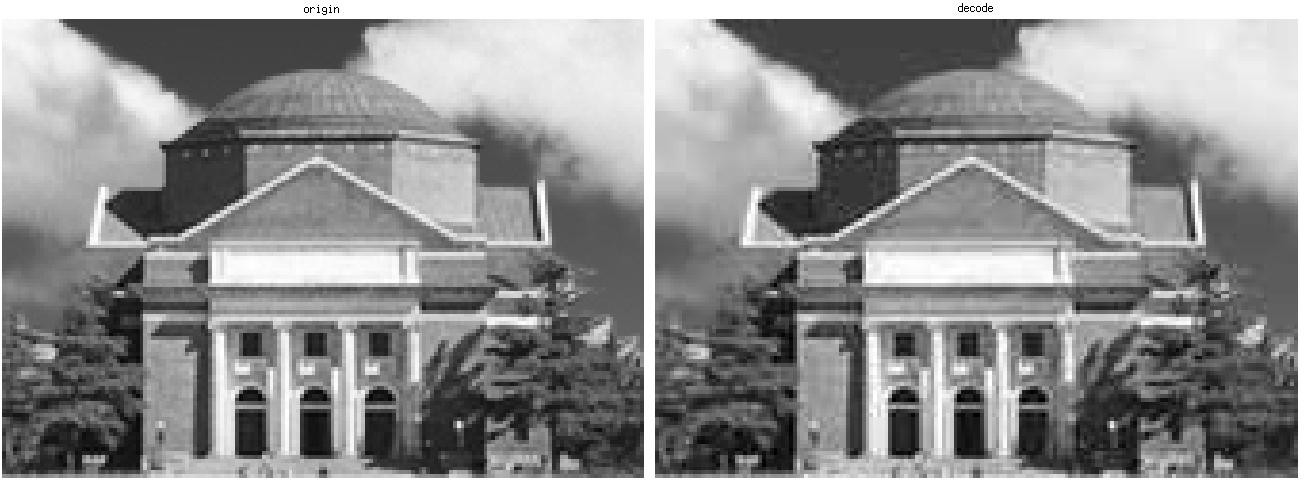
\includegraphics[width=0.8\textwidth]{a3_2_10.jpg}\\
    \caption{原图与编码解码后的图像\label{a3210}}
\end{figure}

代码如下(a3\_2\_10.m):
\lstinputlisting[language=matlab]{a3_2_10.m}

\subsection{
将量化步长减小为原来的一半,重故编解码。同标准量化步长的情况比
较压缩比和图像质量。
}
使QTAB=QTAB./2即可。肉眼难以看到变化,压缩比为4.4081,PSNR为37.32。

\subsection{
 看电视时偶尔能看到美丽的雪花图像(见 snow.mat),请对其编解码。
和测试图像的压缩比和图像质量进行比较,并解释比较结果。
}
如图\ref{a312},把hall\_gray换成snow即可,得到压缩比为3.6407,PSNR=29.5614。两者看起来很像,但编码解码后的图看起来颗粒要大一些。
这是因为编码过程中滤去了高频分量,是的雪花中一些变化很快的部分不再那么明显。
\begin{figure}
    \centering
    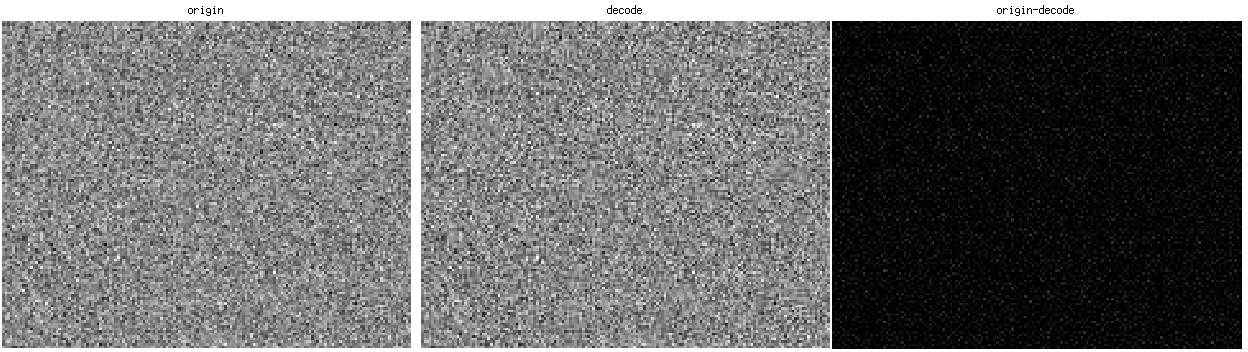
\includegraphics[width=0.8\textwidth]{a3_2_12.jpg}\\
    \caption{雪花原图、编码后的图像和两者的差\label{a3212}}
\end{figure}

\section{信息隐藏}
\subsection{实现本章介绍的空域隐藏方法和提取方法。验证其抗JPEG编码能力。}    
这里采用了空域隐藏可以直接恢复\footnote{只处理了8bit,也就是只有英文字符,虽然增加每个字符的bit数可以加密更多的字符,这里不对字符集进行进一步的探讨}原始信息 A quick brown fox jump over the lazy dog。但是jpeg编码解码后再解密就变成了乱码。

\subsection{
}
\end{document}
